\documentclass[presentation]{beamer}


%%% Packages.

\usepackage[utf8]{inputenc}
\usepackage[T1]{fontenc}
\usepackage{fixltx2e}
\usepackage{graphicx}
\usepackage{longtable}
\usepackage{float}
\usepackage{wrapfig}
\usepackage{rotating}
\usepackage[normalem]{ulem}
\usepackage{amsmath, amssymb}
\usepackage{textcomp}
\usepackage{marvosym}
\usepackage{wasysym}
\usepackage{hyperref}
\tolerance=1000
\usepackage[english, russian]{babel}
\usepackage[labelformat=empty]{caption}
\usepackage{subcaption}
\usepackage{listings}
\usepackage{color}
\let\Cross\relax
\let\Square\relax
\usepackage{bbding}


%%% 

\graphicspath{{graphics/}}

\usetheme[height=20pt]{Rochester}


%%% Title.

\author{Артём Попцов}
\date{2015-10-24}

\title{Git}

\begin{document}

\maketitle


%%% TOC.

\begin{frame}{Содержание}
  \setcounter{tocdepth}{1}
  \tableofcontents
\end{frame}


%%% 

\section{Ветвление}

\subsection{Ветвление}

\begin{frame}{Ветвление}
  \begin{columns}
    \begin{column}{0.5\textwidth}
      \raisebox{-.30em}{\Large\HandRight}\hspace{.25em} Ветвь
      (англ. \emph{branch}) -- направление разработки, независимое от
      других. \newline

      Ветви создаются для:
      \begin{itemize}
        \item Параллельной работы над разными частями проекта
        \item Выпуска стабильных релизов проекта
        \item Тестирования ``потенциально опасных'' идей
      \end{itemize}
    \end{column}
    \begin{column}{0.5\textwidth}
      \begin{figure}[htb]
        \centering
        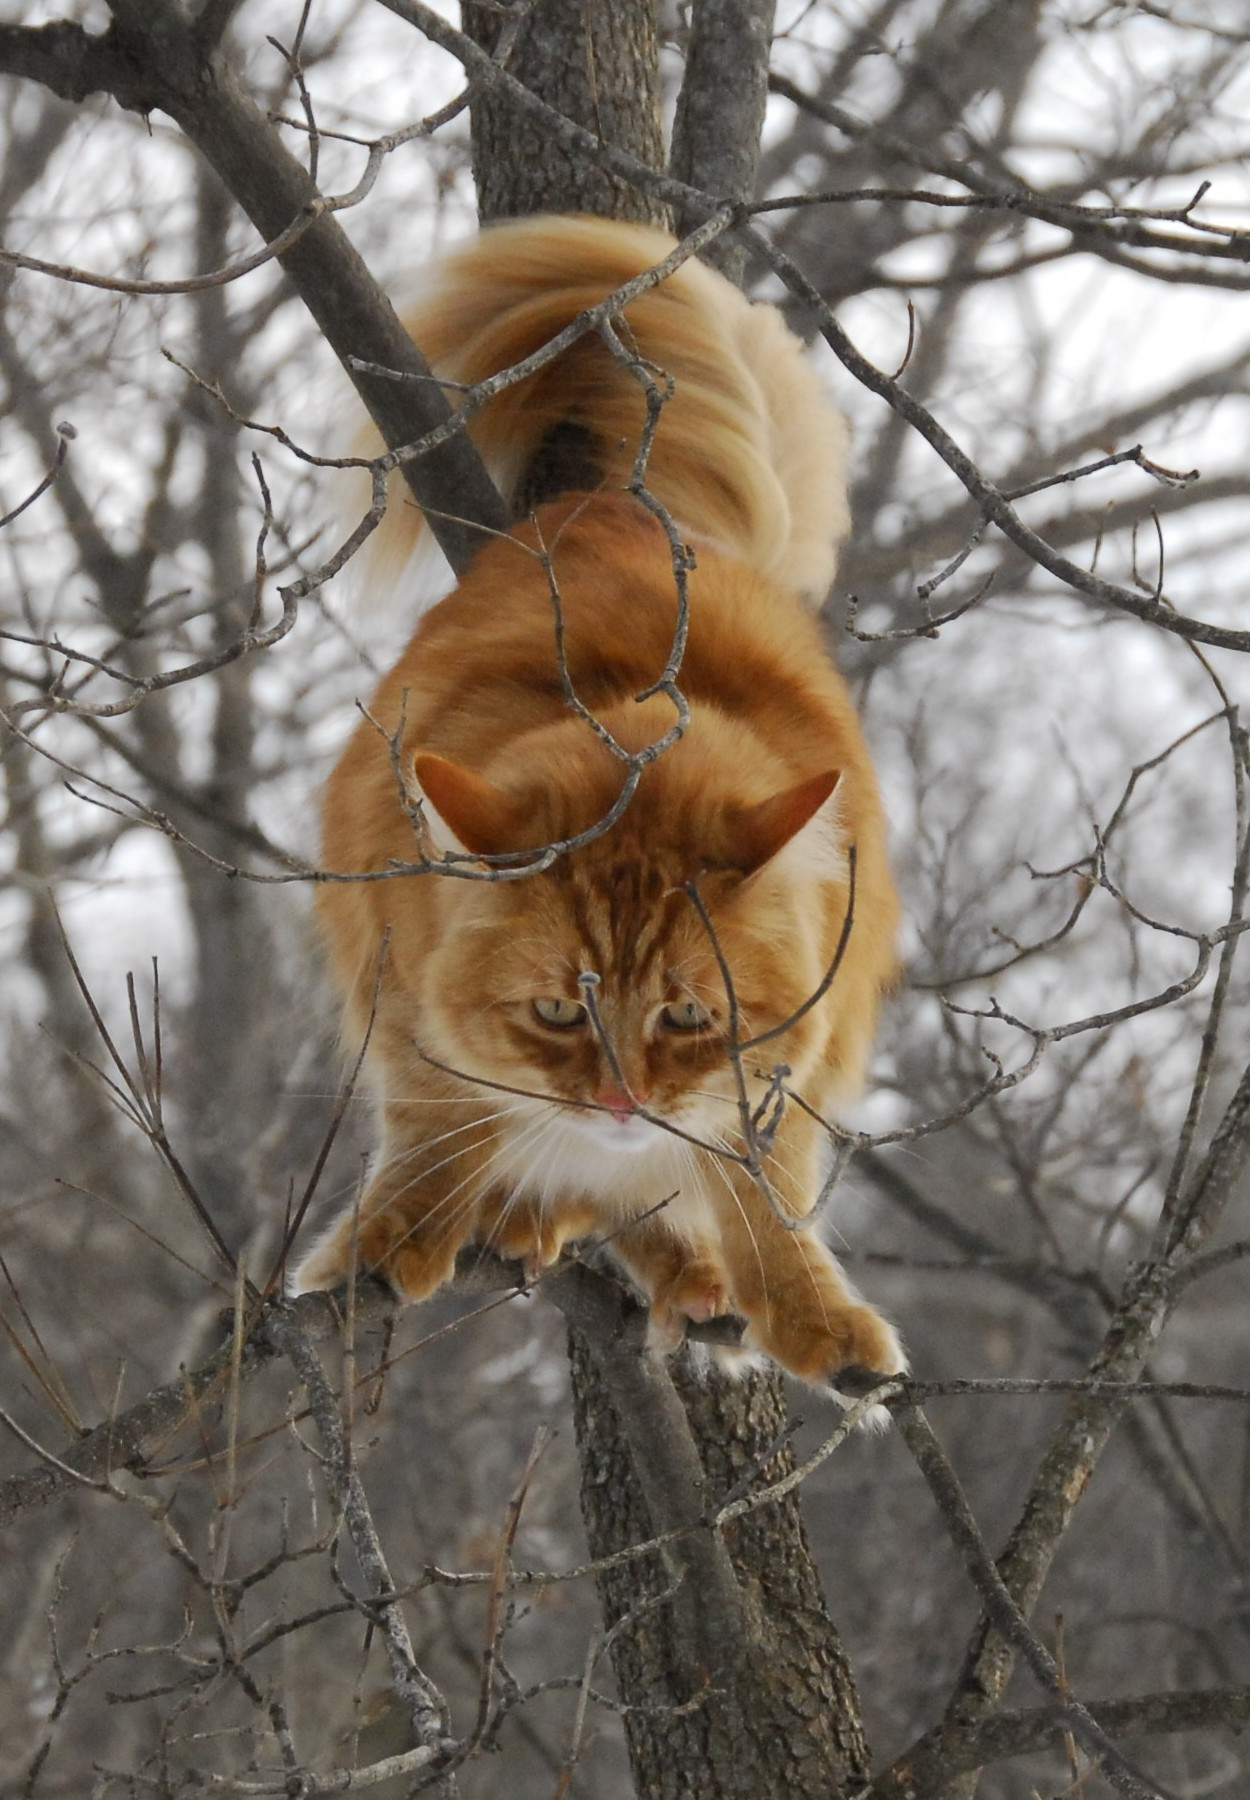
\includegraphics[width=.9\textwidth]{cat-on-branches}
        \newline Мастер ветвления
      \end{figure}
    \end{column}
  \end{columns}
\end{frame}


\begin{frame}[fragile]{Создание ветви -- 1}
  \begin{columns}
    \begin{column}{.6\textwidth}
      Создадим тестовый проект: \newline
\begin{verbatim}
$ cd ~/src/my-project
$ git init
$ git add hello-world.txt
$ git commit -m "Initial commit"
  ... меняем hello-world.txt ...
$ git add hello-world.txt
$ git commit \
    -m "hello-world.txt: Update"
\end{verbatim}
      \end{column}
      \begin{column}{.4\textwidth}
        \begin{figure}[htb]
          \centering
          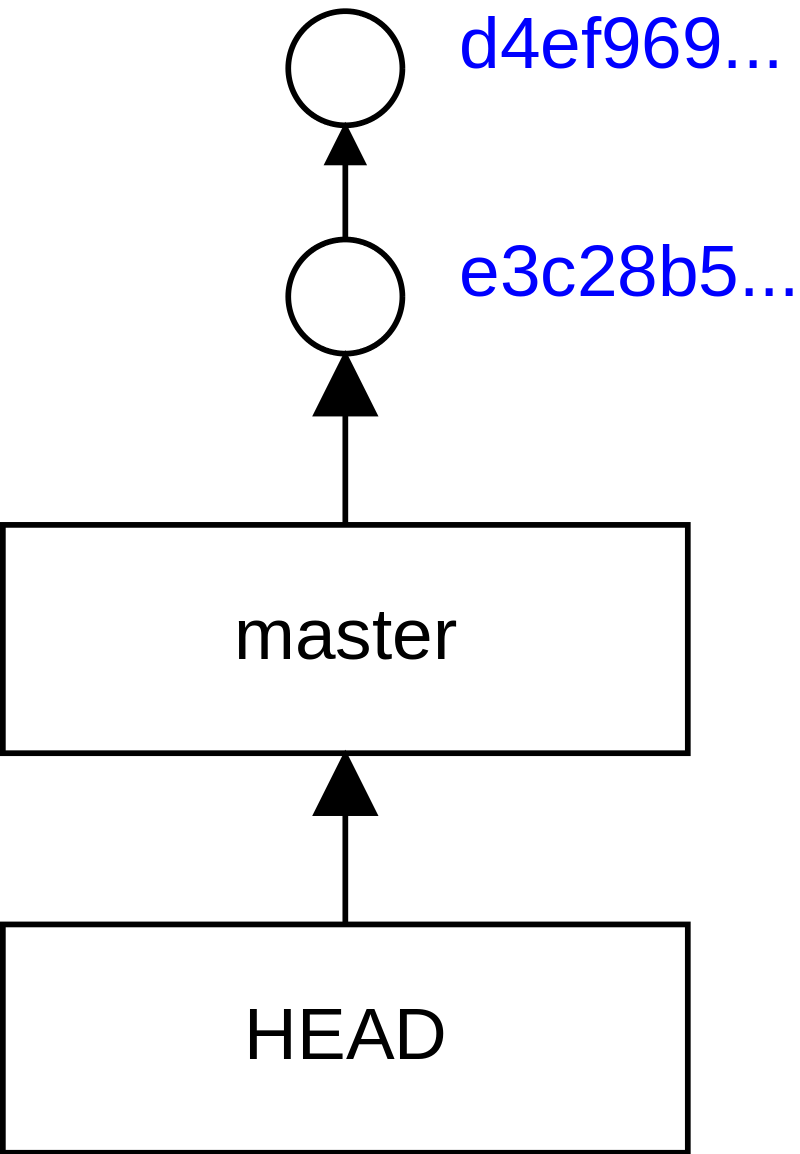
\includegraphics[height=.7\textheight]{git-basics-1}
        \end{figure}
      \end{column}
    \end{columns}
\end{frame}

\begin{frame}[fragile]{Создание ветви -- 2}
  \begin{columns}
    \begin{column}{.6\textwidth}
      Теперь создадим ветвь:
\begin{verbatim}
$ git branch branch-1
\end{verbatim}

      Переключимся на новую ветвь:
\begin{verbatim}
$ git checkout branch-1
\end{verbatim}
      \ldots{}\newline\newline
      Тоже, что описано выше, но одной командой:
\begin{verbatim}
$ git checkout -b branch-1
\end{verbatim}
      \end{column}
      \begin{column}{.4\textwidth}
        \begin{figure}[htb]
          \centering
          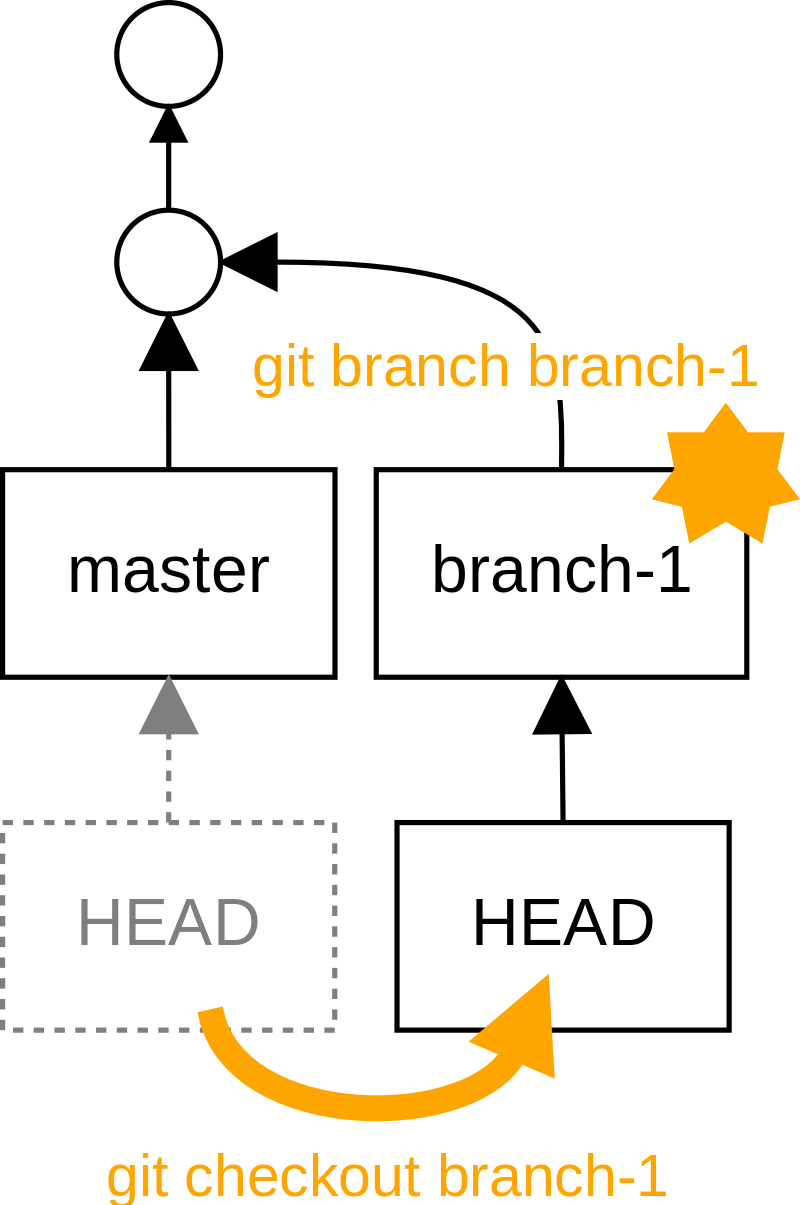
\includegraphics[height=.7\textheight]{git-operation-branch-1}
        \end{figure}
      \end{column}
    \end{columns}
\end{frame}

\begin{frame}[fragile]{Как работает \texttt{git checkout}}
  \begin{columns}
    \begin{column}{.6\textwidth}
      \texttt{git checkout branch-1} делает две вещи:
      \begin{enumerate}
      \item Копирует в рабочий каталог файлы с верхушки ветви
      \item Перемещает указатель \texttt{HEAD} на ветвь
      \end{enumerate}
    \end{column}
      \begin{column}{.4\textwidth}
        \begin{figure}[htb]
          \centering
          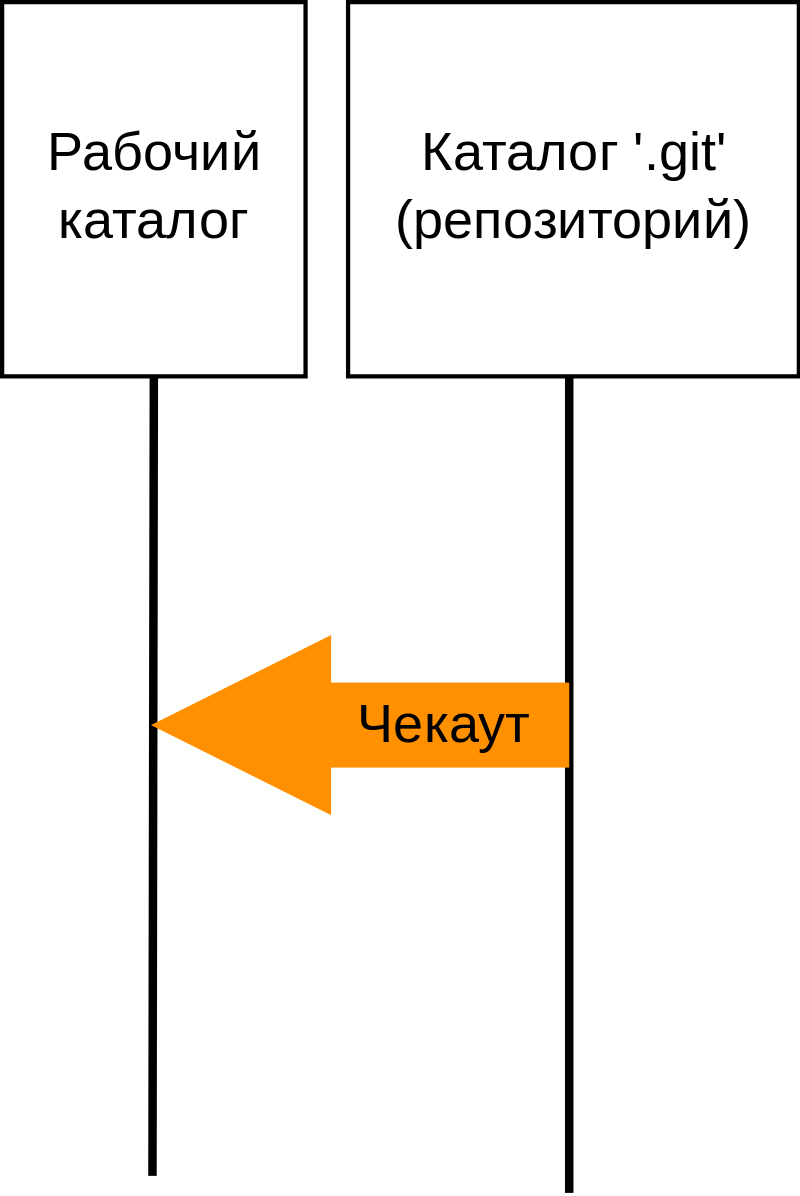
\includegraphics[height=.7\textheight]{git-operation-checkout-file}
        \end{figure}
      \end{column}
    \end{columns}
\end{frame}


\begin{frame}[fragile]{Параллельная разработка -- 1}
  \begin{columns}
    \begin{column}{.5\textwidth}
      \begin{enumerate}
      \item \textbf{Меняем \texttt{hello-world.txt}}
      \item \textbf{Фиксируем изменения:}
\begin{verbatim}
$ git commit
\end{verbatim}
      \end{enumerate}
      \end{column}
      \begin{column}{.5\textwidth}
        \begin{figure}[htb]
          \centering
          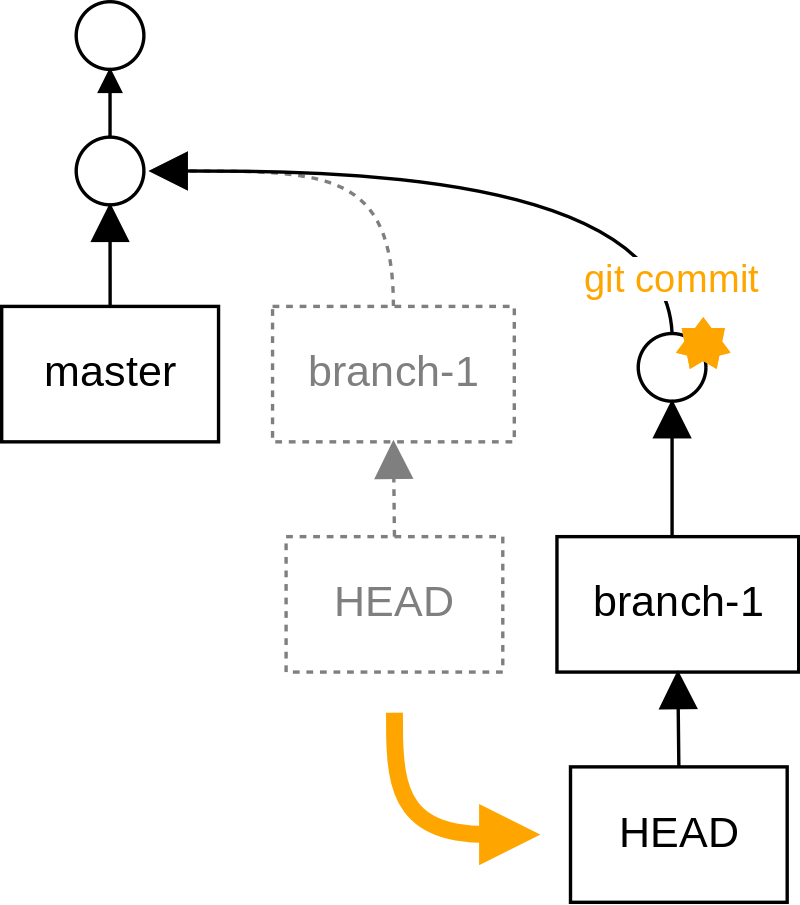
\includegraphics[height=.7\textheight]{git-operation-branch-2}
        \end{figure}
      \end{column}
    \end{columns}
\end{frame}

\begin{frame}[fragile]{Параллельная разработка -- 2}
  \begin{columns}
    \begin{column}{.5\textwidth}
      \begin{enumerate}
      \item Меняем \texttt{hello-world.txt}
      \item Фиксируем изменения:
\begin{verbatim}
$ git commit
\end{verbatim}
      \item \textbf{Переходим на ветвь \texttt{master}:}
\begin{verbatim}
$ git checkout master
\end{verbatim}
      \end{enumerate}
      \end{column}
      \begin{column}{.5\textwidth}
        \begin{figure}[htb]
          \centering
          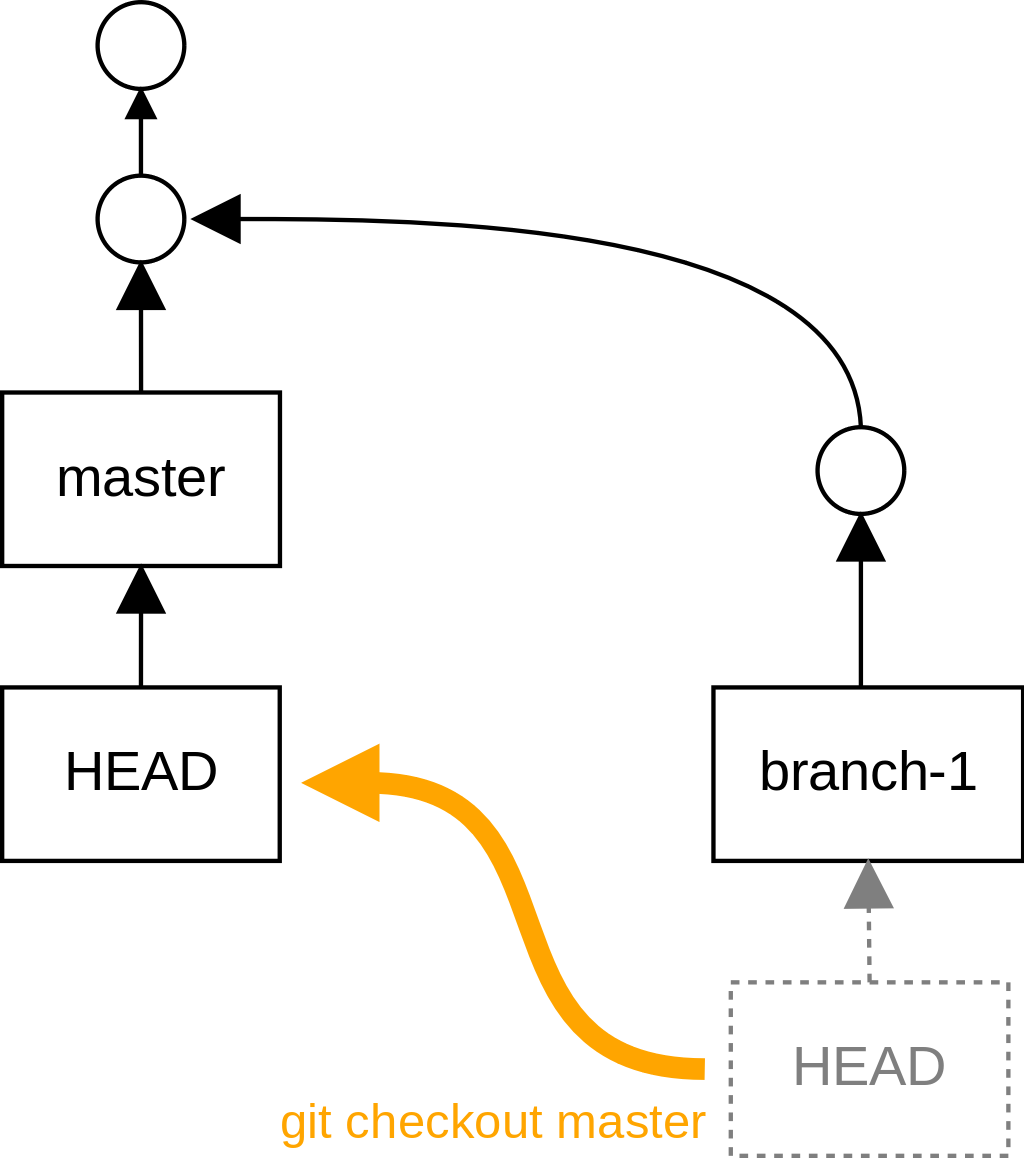
\includegraphics[height=.7\textheight]{git-operation-branch-3}
        \end{figure}
      \end{column}
    \end{columns}
\end{frame}

\begin{frame}[fragile]{Параллельная разработка -- 3}
  \begin{columns}
    \begin{column}{.5\textwidth}
      \begin{enumerate}
      \item Меняем \texttt{hello-world.txt}
      \item Фиксируем изменения:
\begin{verbatim}
$ git commit
\end{verbatim}
      \item Переходим на ветвь \texttt{master}:
\begin{verbatim}
$ git checkout master
\end{verbatim}
      \item \textbf{Меняем \texttt{hello-world.txt}}
      \item \textbf{Фиксируем изменения:}
\begin{verbatim}
$ git commit
\end{verbatim}
      \end{enumerate}
      \end{column}
      \begin{column}{.5\textwidth}
        \begin{figure}[htb]
          \centering
          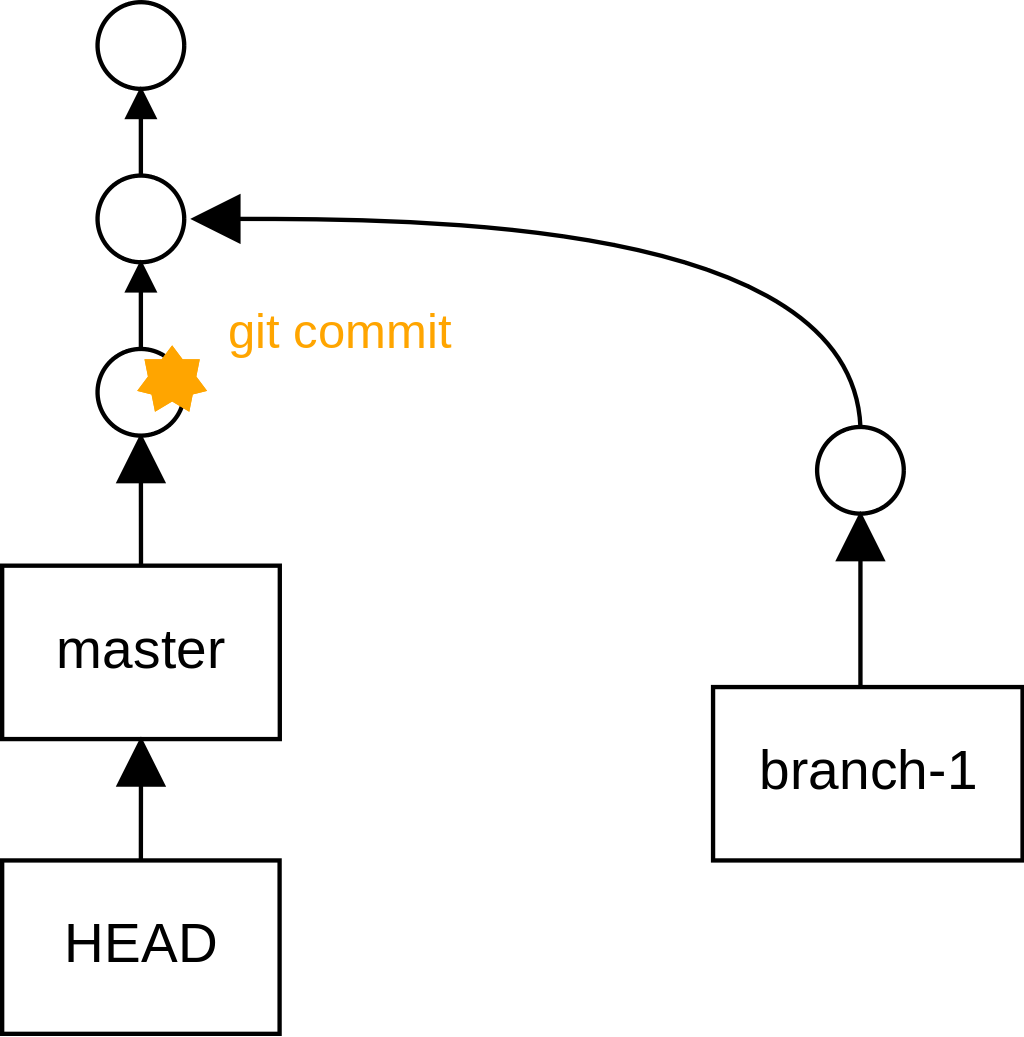
\includegraphics[height=.7\textheight]{git-operation-branch-4}
        \end{figure}
      \end{column}
    \end{columns}
\end{frame}


%%%

\section{Слияние}

\subsection{Слияние}

\begin{frame}{Слияние}
  \begin{columns}
    \begin{column}{.5\textwidth}
      \raisebox{-.30em}{\Large\HandRight}\hspace{.25em} Слияние
      (англ. \emph{merge}) -- объединение изменений из нескольких
      источников.\newline\newline

      К примеру: слияние (``мёрж'') двух ветвей.\newline\newline
      
      Типы слияния:
      \begin{itemize}
      \item fast-forward
      \item Остальные  ;-)
      \end{itemize}
    \end{column}
      \begin{column}{.5\textwidth}
        \begin{figure}[htb]
          \centering
          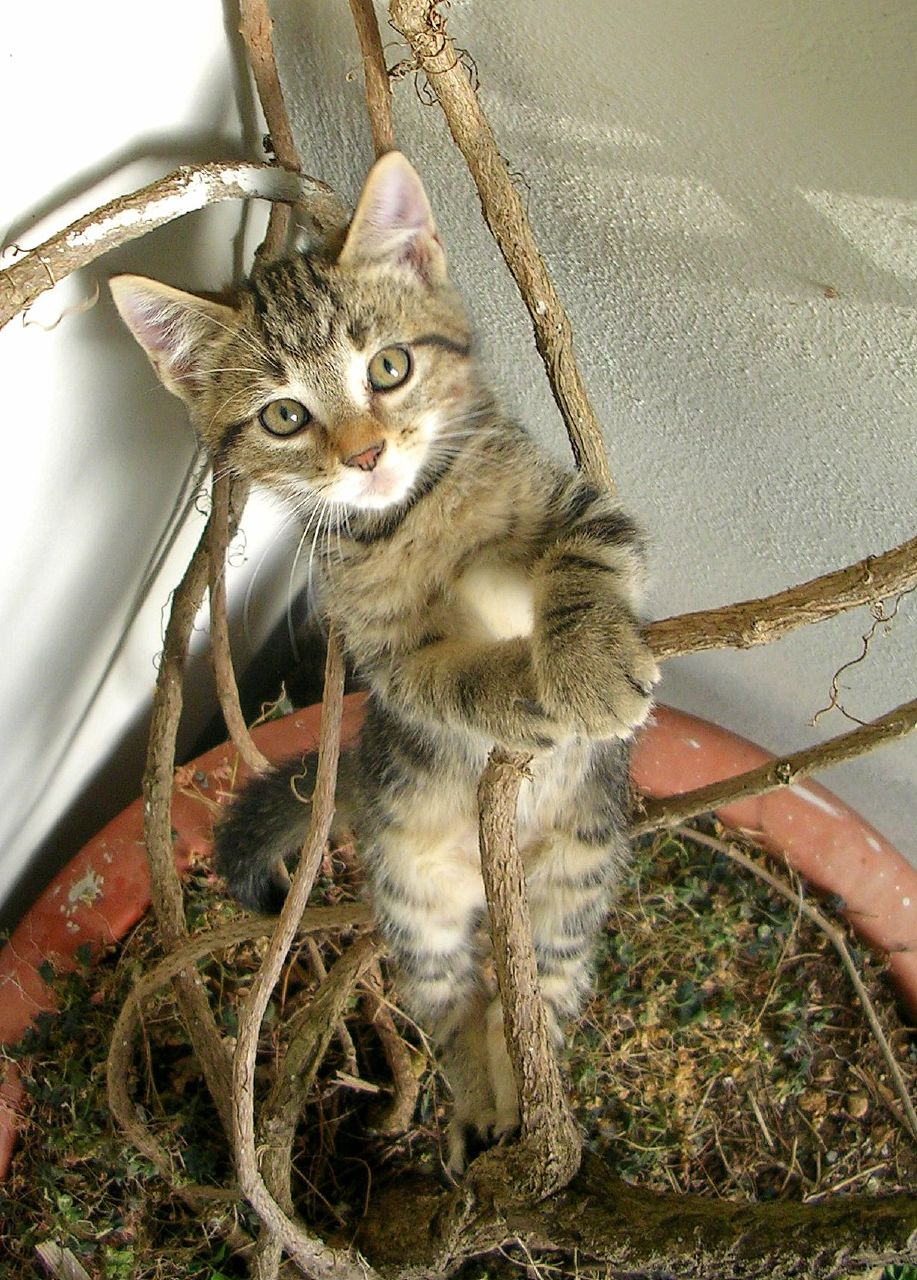
\includegraphics[height=.8\textheight]{Fazen_-_charming_(by)}
          \newline
          Ну что, мёржим?
        \end{figure}
      \end{column}
    \end{columns}
\end{frame}

\begin{frame}[fragile]{Простое слияние: fast-forward -- 1}
  \begin{columns}
    \begin{column}{.4\textwidth}
      Начальное состояние:
      \begin{itemize}
      \item На \texttt{branch-1} закоммичены (зафиксированы) изменения
      \item \texttt{master} не двигался с момента создания ветви
        \texttt{branch-1}
      \end{itemize}
      \end{column}
      \begin{column}{.6\textwidth}
        \begin{figure}[htb]
          \centering
          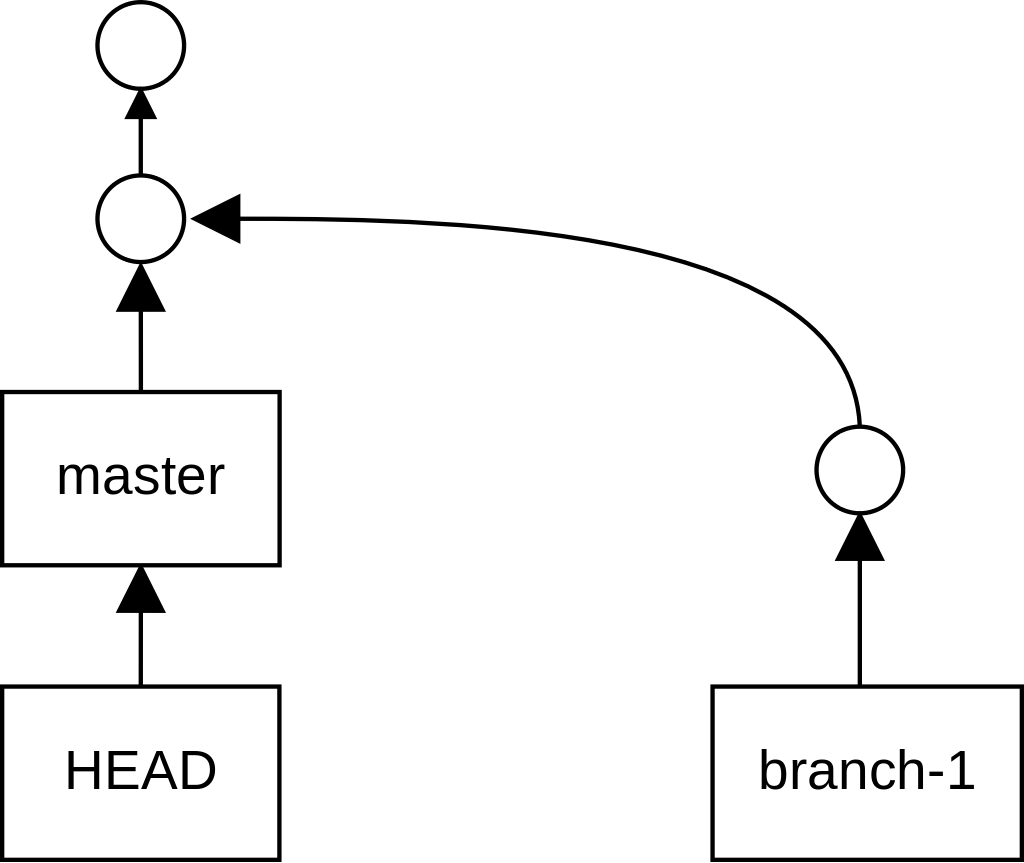
\includegraphics[height=.6\textheight]{git-operation-merge-1-1}
        \end{figure}
      \end{column}
    \end{columns}
\end{frame}

\begin{frame}[fragile]{Простое слияние: fast-forward -- 2}
  \begin{columns}
    \begin{column}{.4\textwidth}
\begin{verbatim}
$ git checkout master
$ git merge branch-1
\end{verbatim}
      Результат:
      \begin{itemize}
      \item Перемещается указатель на верхушку ветви
      \item Новых коммитов не создаётся
      \end{itemize}
      \end{column}
      \begin{column}{.6\textwidth}
        \begin{figure}[htb]
          \centering
          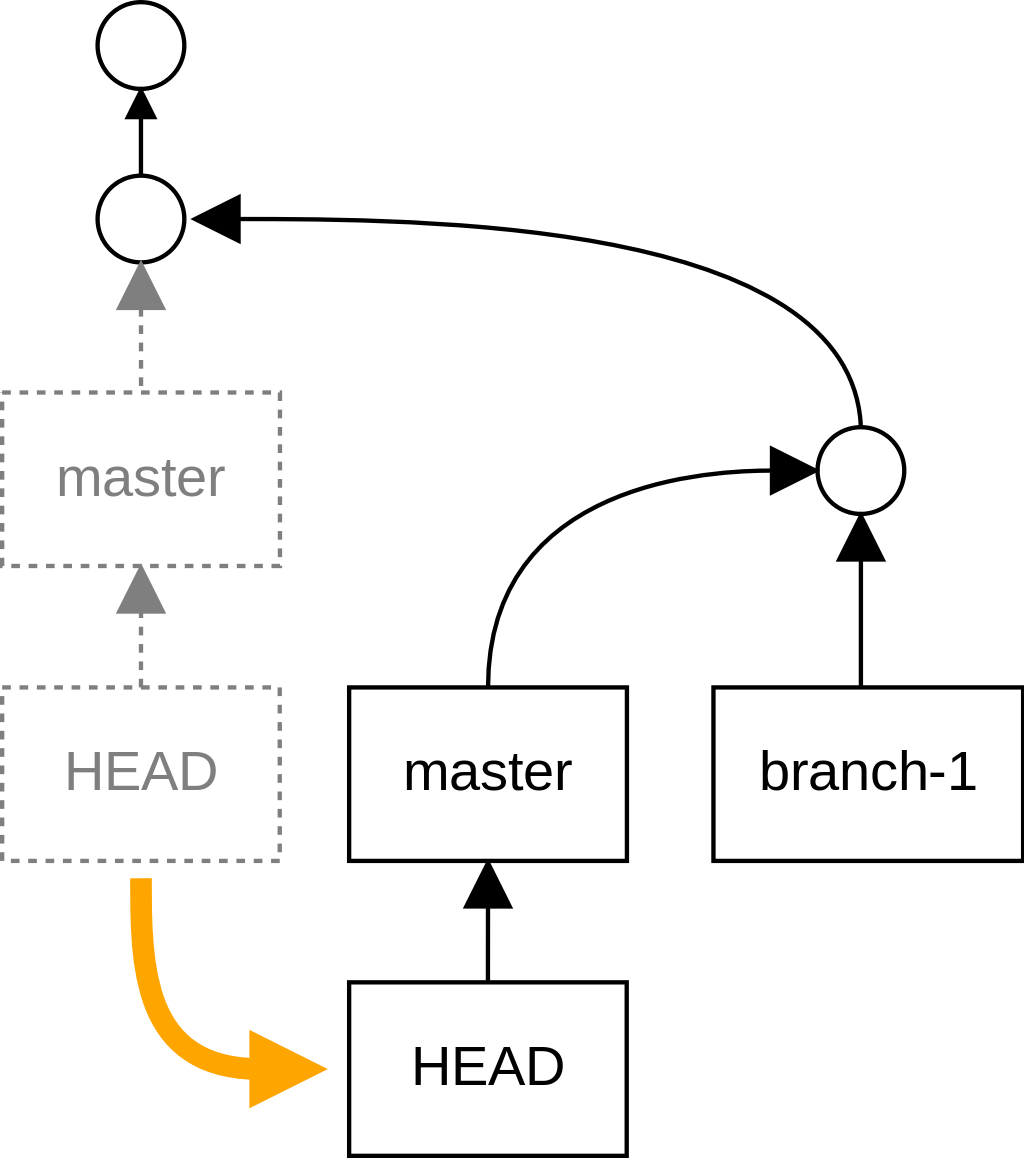
\includegraphics[height=.7\textheight]{git-operation-merge-1}
        \end{figure}
      \end{column}
    \end{columns}
\end{frame}

\begin{frame}[fragile]{Простое слияние: fast-forward -- 3}
  \begin{columns}
    \begin{column}{.4\textwidth}
\begin{verbatim}
$ git checkout master
$ git merge branch-1
\end{verbatim}
      Результат:
      \begin{itemize}
      \item Перемещается указатель на верхушку ветви
      \item Новых коммитов не создаётся
      \end{itemize}
      \end{column}
      \begin{column}{.6\textwidth}
        \begin{figure}[htb]
          \centering
          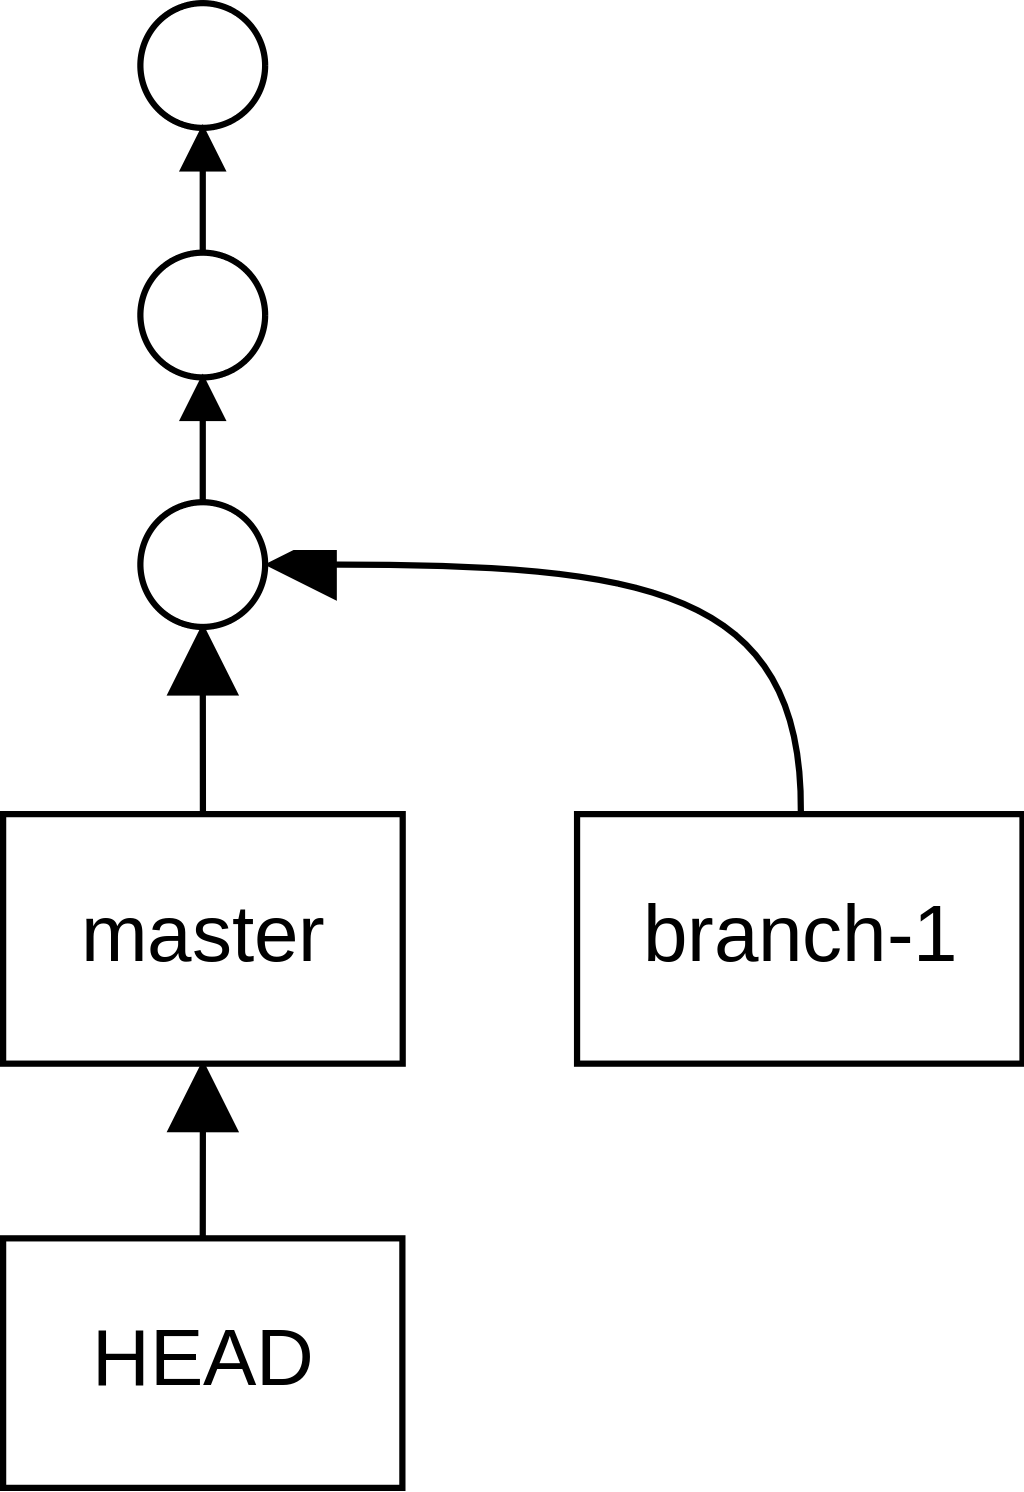
\includegraphics[height=.7\textheight]{git-operation-merge-1-2}
        \end{figure}
      \end{column}
    \end{columns}
\end{frame}

\begin{frame}[fragile]{Удаление ветви}
  \begin{columns}
    \begin{column}{.4\textwidth}
\begin{verbatim}
$ git branch --delete branch-1
\end{verbatim}
      Результат:
      \begin{itemize}
      \item Ветвь \texttt{branch-1} удалена
      \end{itemize}
        \begin{figure}[htb]
          \centering
          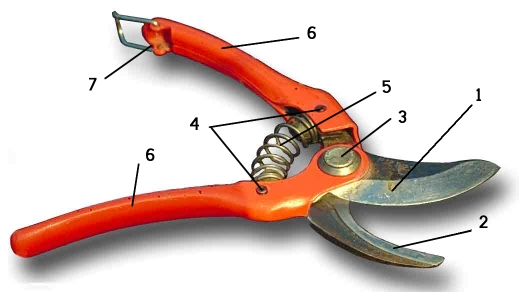
\includegraphics[height=.7\textwidth]{Sekator_shema}
        \end{figure}
      \end{column}
      \begin{column}{.6\textwidth}
        \begin{figure}[htb]
          \centering
          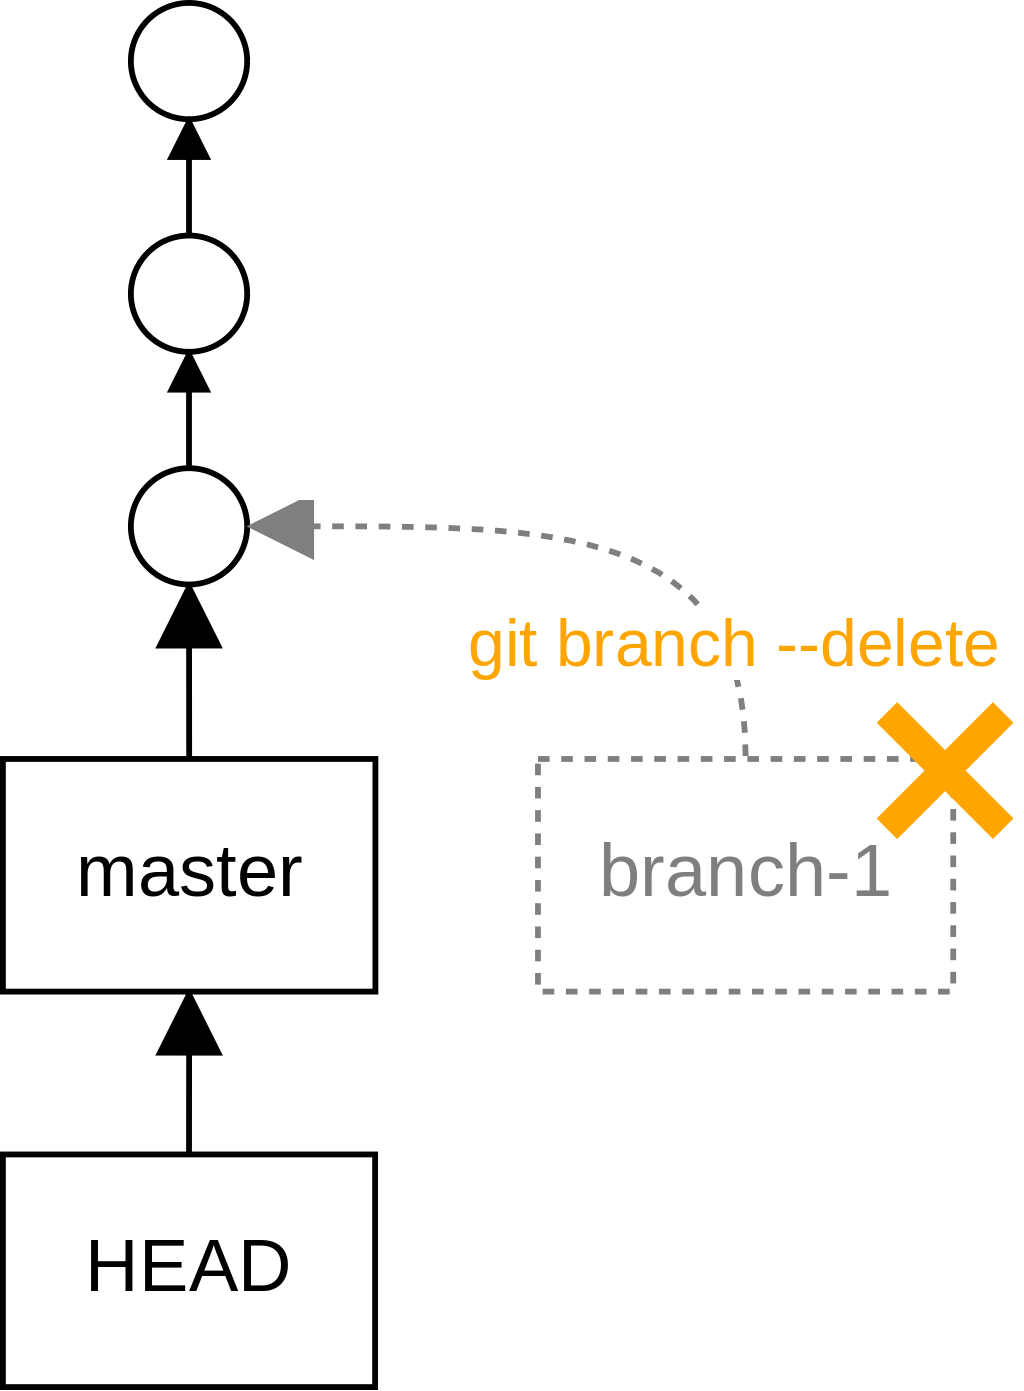
\includegraphics[height=.7\textheight]{git-operation-merge-1-3}
        \end{figure}
      \end{column}
    \end{columns}
\end{frame}


\begin{frame}[fragile]{"Тяжёлый случай": recursive merge -- 1}
  \begin{columns}
    \begin{column}{.4\textwidth}
      Начальное состояние:
      \begin{itemize}
      \item На \texttt{branch-1} закоммичены (зафиксированы) изменения
      \item На \texttt{master} закоммичены изменения после создания
        ветви \texttt{branch-1}
      \item Изменения на ветвях не пересекаются (сделаны в разных файлах)
      \end{itemize}
      \end{column}
      \begin{column}{.6\textwidth}
        \begin{figure}[htb]
          \centering
          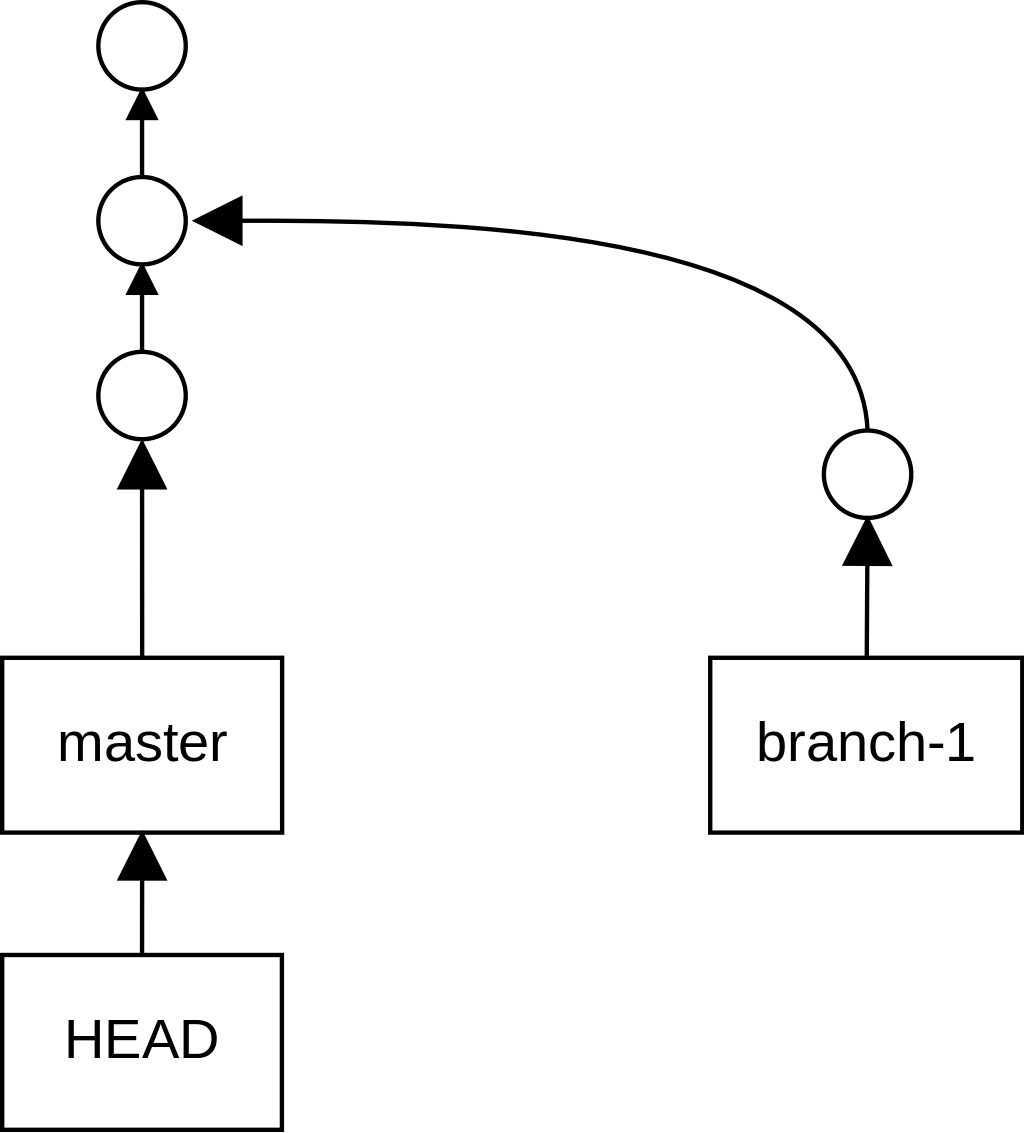
\includegraphics[height=.7\textheight]{git-operation-merge-2-1}
        \end{figure}
      \end{column}
    \end{columns}
\end{frame}

\begin{frame}[fragile]{"Тяжёлый случай": recursive merge -- 2}
  \begin{columns}
    \begin{column}{.4\textwidth}
\begin{verbatim}
$ git checkout master
$ git merge branch-1
\end{verbatim}
      Результат:
      \begin{itemize}
      \item Производится попытка автоматического слияния изменений
      \item Результатом слияния является новый коммит
      \item Перемещается указатель на верхушку ветви
      \end{itemize}
      \end{column}
      \begin{column}{.6\textwidth}
        \begin{figure}[htb]
          \centering
          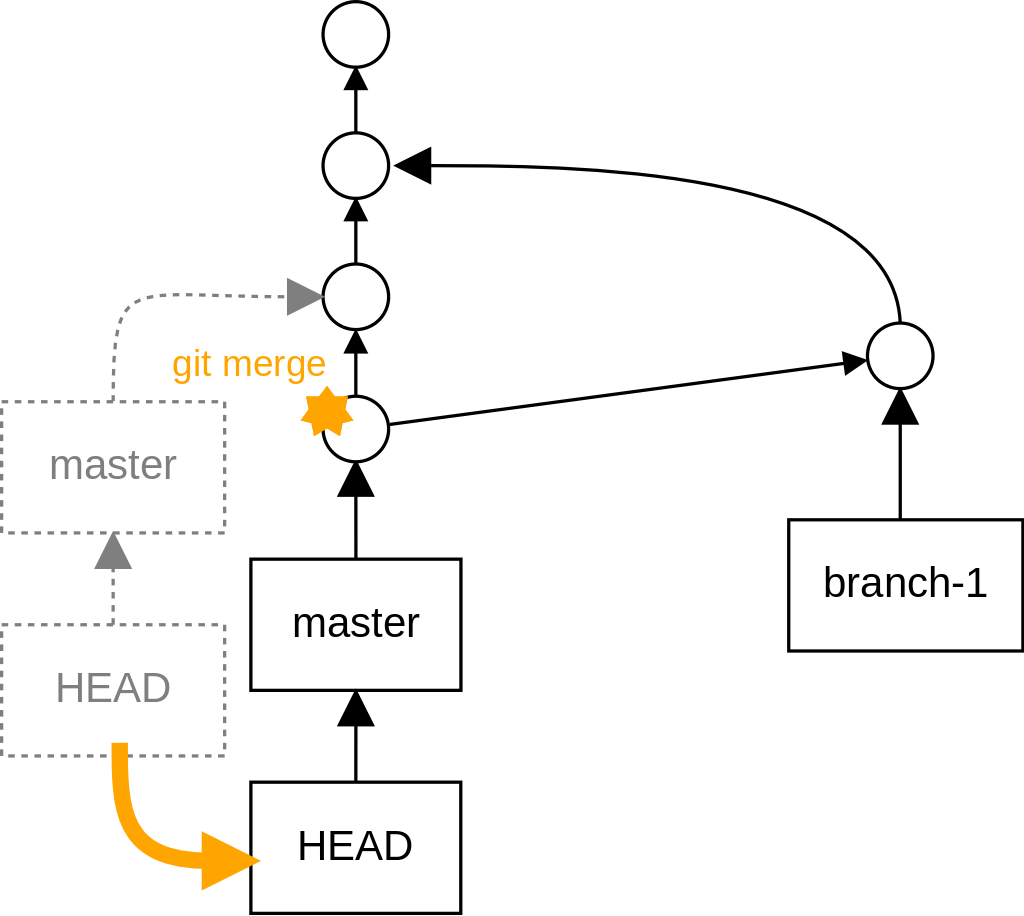
\includegraphics[height=.7\textheight]{git-operation-merge-2-2}
        \end{figure}
      \end{column}
    \end{columns}
\end{frame}

\begin{frame}[fragile]{"Тяжёлый случай": recursive merge -- 3}
  \begin{columns}
    \begin{column}{.4\textwidth}
\begin{verbatim}
$ git branch \
     --delete branch-1
\end{verbatim}
      Результат:
      \begin{itemize}
      \item Ветвь \texttt{branch-1} удалена
      \end{itemize}
      \end{column}
      \begin{column}{.6\textwidth}
        \begin{figure}[htb]
          \centering
          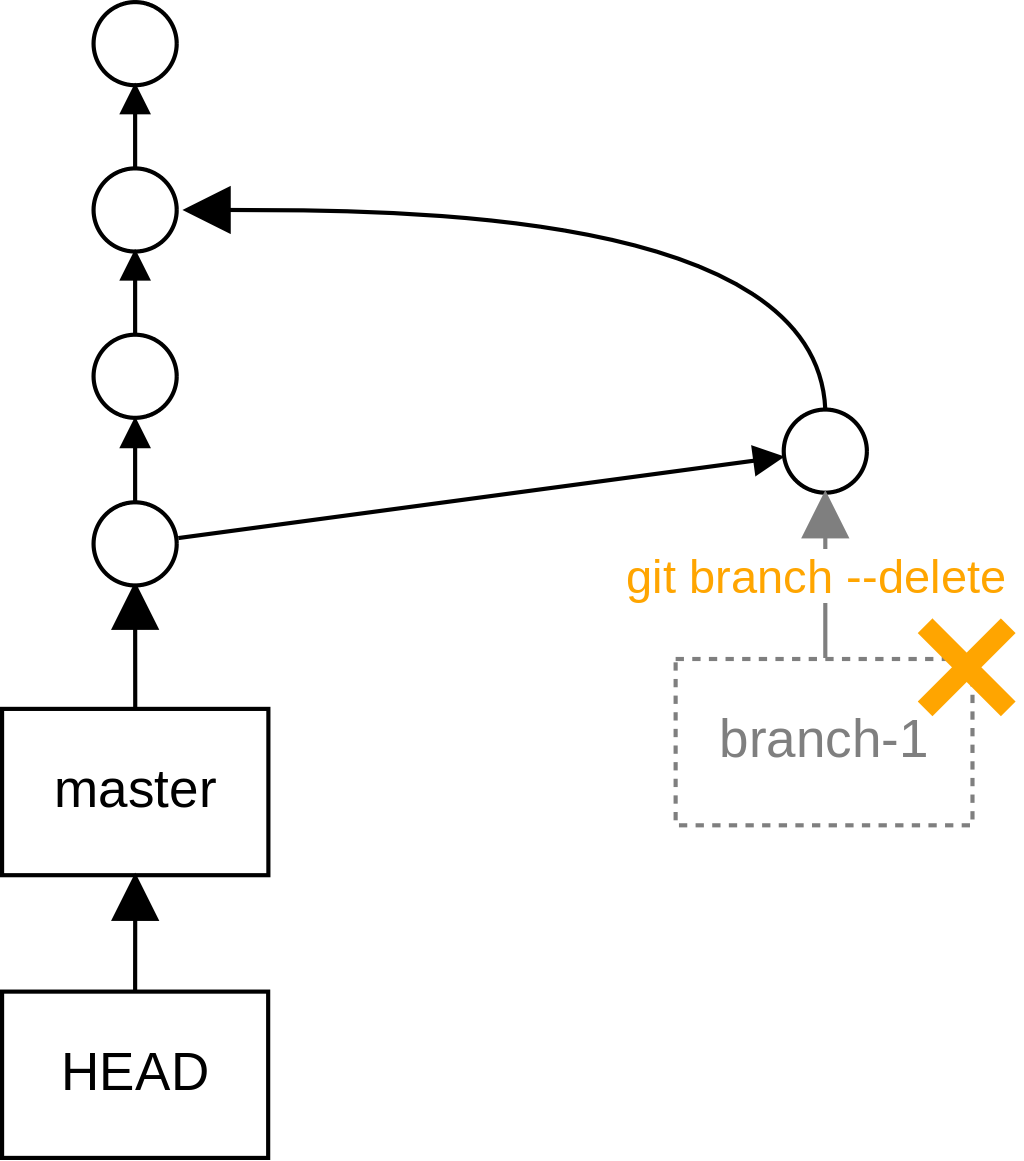
\includegraphics[height=.7\textheight]{git-operation-merge-2-3}
        \end{figure}
      \end{column}
    \end{columns}
\end{frame}

\begin{frame}[fragile]{Шпаргалка садовника}
  \begin{columns}
    \begin{column}{.6\textwidth}
      \begin{itemize}
      \item Создать ветвь и переключиться на неё:
\begin{verbatim}
$ git checkout -b branch-1
\end{verbatim}
      \item Замёржить ветвь \texttt{branch-1} на \texttt{master}:
\begin{verbatim}
$ git checkout master
$ git merge branch-1
\end{verbatim}
      \item Удалить ветвь \texttt{branch-1}:
\begin{verbatim}
$ git branch --delete branch-1
\end{verbatim}
      \item Показать список ветвей:
\begin{verbatim}
$ git branch
\end{verbatim}
      \end{itemize}
    \end{column}
    \begin{column}{.4\textwidth}
      \begin{figure}[htb]
        \centering
        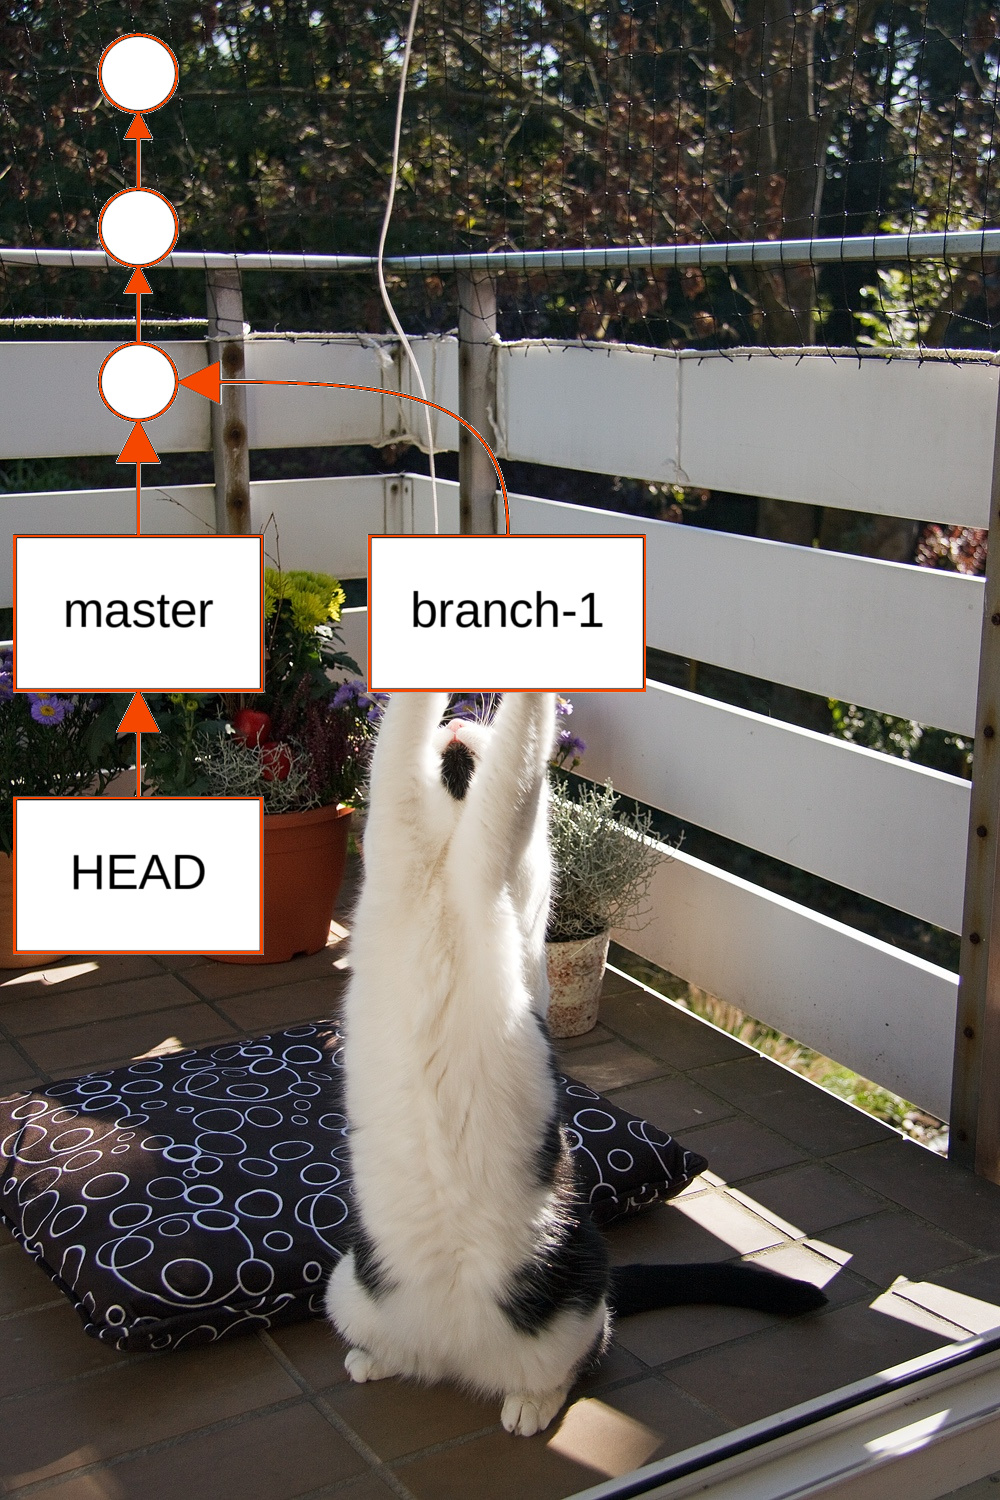
\includegraphics[height=.8\textheight]{cat-gitbranching}
      \end{figure}
    \end{column}
  \end{columns}
\end{frame}


\begin{frame}[fragile]{Разрешение конфликтов -- 1}
  \begin{columns}
    \begin{column}{.6\textwidth}
\begin{verbatim}
$ git init

$ echo "hello" > hello-world.txt
$ git add hello-world.txt
$ git commit

$ git checkout -b branch-1
$ echo "world" >> hello-world.txt
$ git add hello-world.txt
$ git commit

$ git checkout master 
$ echo "git" >> hello-world.txt
$ git add hello-world.txt
$ git commit
\end{verbatim}
      \end{column}
      \begin{column}{.4\textwidth}
        \begin{figure}[htb]
          \centering
          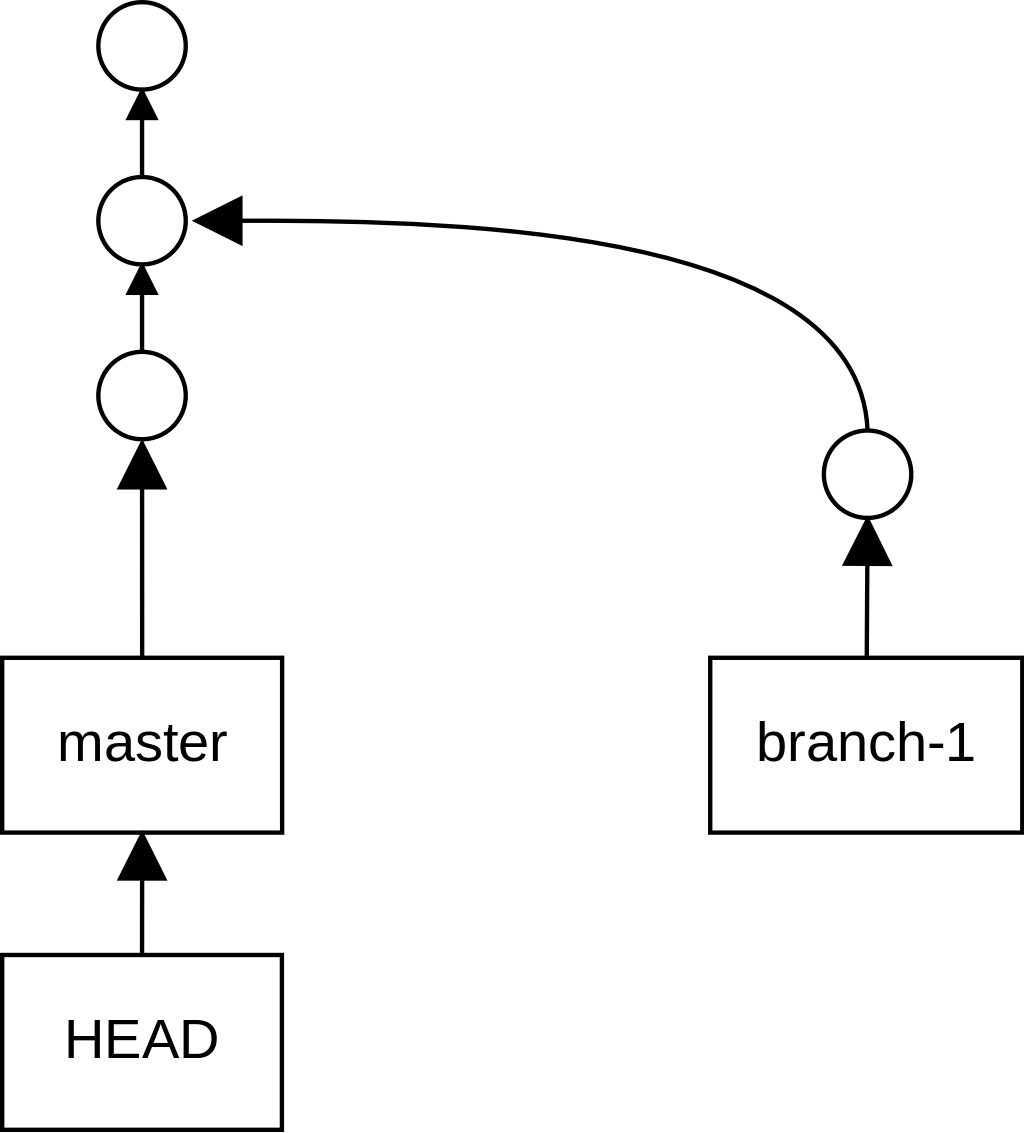
\includegraphics[height=.6\textheight]{git-operation-merge-2-1}
        \end{figure}
      \end{column}
    \end{columns}
\end{frame}

\begin{frame}[fragile]{Разрешение конфликтов -- 2}
  \begin{columns}
    \begin{column}{.6\textwidth}
      Начальное состояние:
      \begin{itemize}
      \item На \texttt{branch-1} закоммичены (зафиксированы) изменения
      \item На \texttt{master} закоммичены изменения после создания
        ветви \texttt{branch-1}
      \item Изменения на ветвях пересекаются (изменены одни и те же
        файлы)
      \end{itemize}
      \end{column}
      \begin{column}{.4\textwidth}
        \begin{figure}[htb]
          \centering
          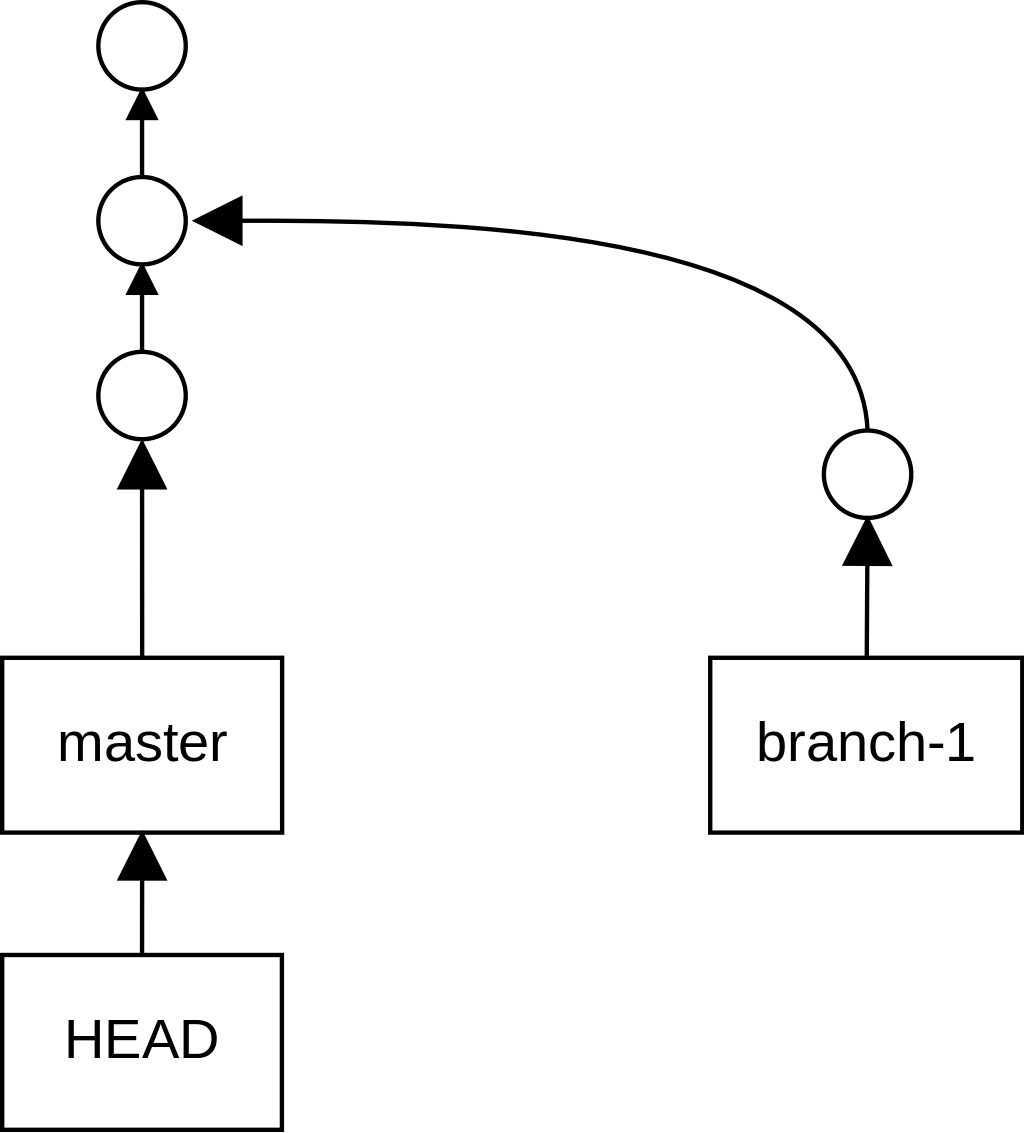
\includegraphics[height=.6\textheight]{git-operation-merge-2-1}
        \end{figure}
      \end{column}
    \end{columns}
\end{frame}

\begin{frame}[fragile]{Разрешение конфликтов -- 3}
  \begin{columns}
    \begin{column}{.6\textwidth}
\begin{verbatim}
$ git merge branch-1
Auto-merging hello-world.txt
CONFLICT (content): Merge conflict
  in hello-world.txt
Automatic merge failed;
  fix conflicts and then commit
  the result.
\end{verbatim}
      \end{column}
      \begin{column}{.4\textwidth}
        \begin{figure}[htb]
          \centering
          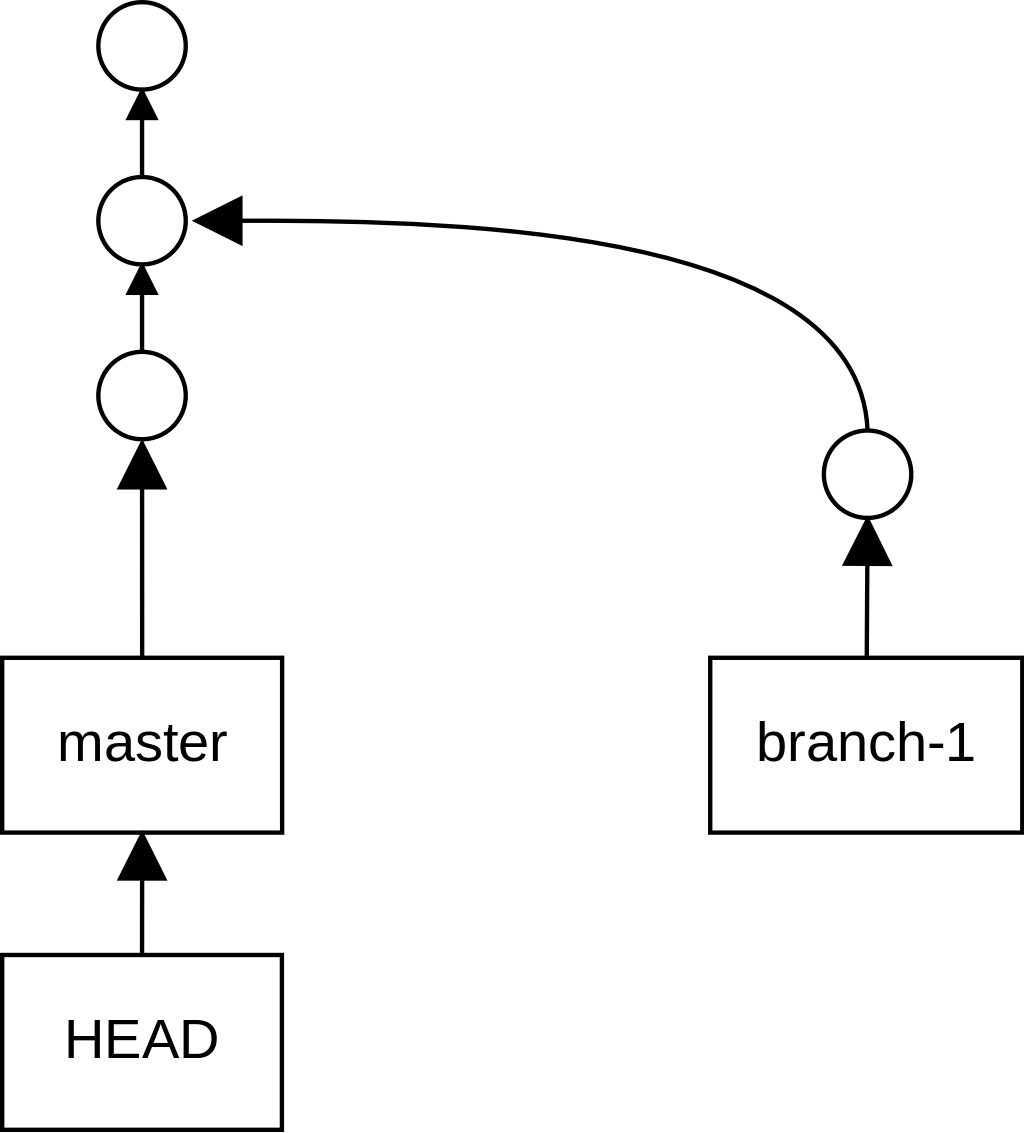
\includegraphics[height=.6\textheight]{git-operation-merge-2-1}
        \end{figure}
      \end{column}
    \end{columns}
\end{frame}

\begin{frame}[fragile]{Разрешение конфликтов -- 4}
  Статус репозитория:
\begin{verbatim}
$ git status
On branch master
You have unmerged paths.
  (fix conflicts and run "git commit")

Unmerged paths:
  (use "git add <file>..." to mark resolution)

	both modified:   hello-world.txt

no changes added to commit (use "git add"
  and/or "git commit -a")
\end{verbatim}
\end{frame}

\begin{frame}[fragile]{Разрешение конфликтов -- 5}
  Файл, в котором возник конфликт, с метками Git:
\begin{verbatim}
$ cat hello-world.txt
hello
<<<<<<< HEAD
git
=======
world
>>>>>>> branch-1
\end{verbatim}
  Разрешаем конфликт вручную, редактируя файл.  Сохраняем.
  Результат:
\begin{verbatim}
$ cat hello-world.txt
hello
git
world
\end{verbatim}
\end{frame}

\begin{frame}[fragile]{Разрешение конфликтов -- 6}
  \begin{columns}
    \begin{column}{.5\textwidth}
      Фиксируем результат слияния:
\begin{verbatim}
$ git add hello-world.txt
$ git commit
\end{verbatim}
      
      Результат:
\begin{verbatim}
$ git log -1
commit ea835e9...
Merge: 35abf34 f3f5057
Author: Artyom V. Poptsov ...
Date:   Fri Aug 26 ...

    Merge branch 'branch-1'
\end{verbatim}
      \end{column}
      \begin{column}{.5\textwidth}
        \begin{figure}[htb]
          \centering
          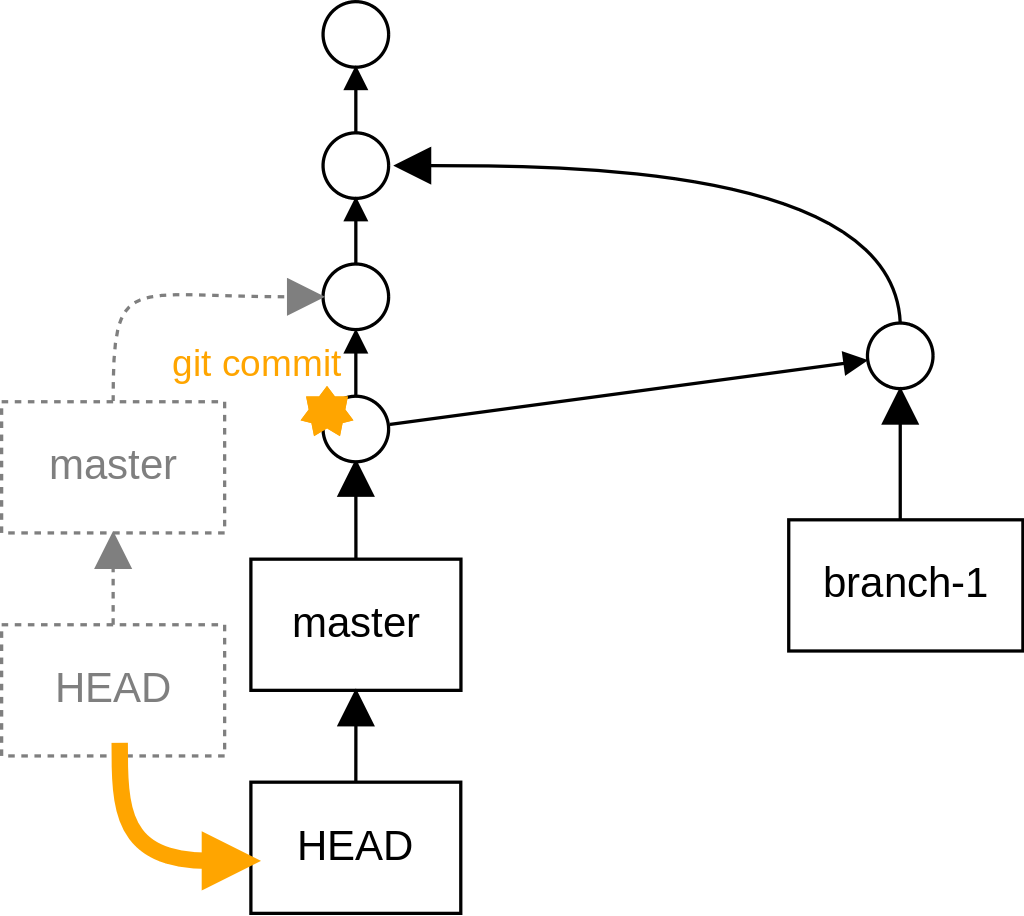
\includegraphics[height=.6\textheight]{git-operation-merge-2-4}
        \end{figure}
      \end{column}
    \end{columns}
\end{frame}


%%%

\section{Редактирование истории}

\subsection{Редактирование истории}


%%%

\section{Полезные трюки}

\subsection{Полезные трюки}


\end{document}

%%%
